% image-kinds-chart — a bar chart rasterised, for image-kinds.tex.
%
% Rendered at 200 dpi to image-kinds-chart.png. Each bar is labelled with its value and each
% axis with its name, so a reader of the image has what it needs to give the table the
% gold file states: no value is hidden in a bar's height alone.
\documentclass[border=6pt]{standalone}
\usepackage{pgfplots}
\pgfplotsset{compat=1.18}
\begin{document}
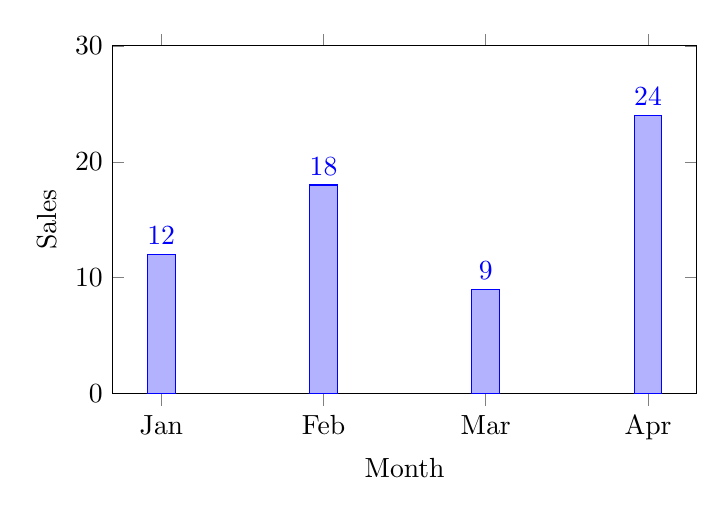
\begin{tikzpicture}
\begin{axis}[ybar, symbolic x coords={Jan,Feb,Mar,Apr}, xtick=data, xlabel={Month}, ylabel={Sales},
    ymin=0, ymax=30, nodes near coords, width=9cm, height=6cm]
\addplot coordinates {(Jan,12) (Feb,18) (Mar,9) (Apr,24)};
\end{axis}
\end{tikzpicture}
\end{document}
